\section{Actualidad}
\label{sec:tics_ACTUALIDAD}

La relación de los videojuegos con la formación surge en los años $90$ y ha
llegado hasta la actualidad en plena efervescencia, siendo aplicados en casi
todos los ámbitos de la educación tanto formal como no formal. Los juegos serios
para el entrenamiento de habilidades se pueden considerar una evolución de las
técnicas de entrenamiento basadas en la realidad virtual que se desarrollaron en
los años 90 y que en la actualidad se han transformado, por su potencial
motivacional, de simulaciones puras a
videojuegos\cite{videojuegos:gonzaleztardon}.


Se presentan varios casos de éxito, donde se puede ver como la utilización de
las \Gls{tic} provocaron un resultado positivo en las personas que lo
utilizaron.

\subsection{Triage Trainer}
	

\begin{description}
\item[Tipo:] Simulación de entrenamiento.
\item[Destinatarios:] Médicos, enfermeros, paramédicos y otros rescatistas.
\item[Contenido:] Entrenamiento para evaluar a los pacientes en un lugar de
    emergencia.
\item[Desarrollador:] \emph{TruSim}
\end{description}

\begin{figure}[h!] 
\centering 
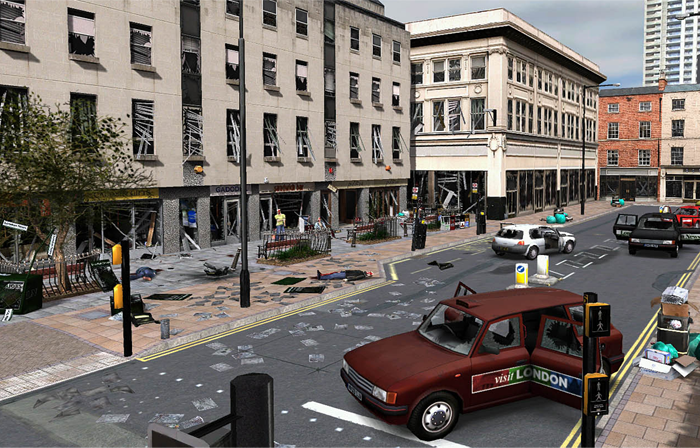
\includegraphics[scale=0.5]{tics/images/triage.png}
\caption{Ambientación de Triage}
\label{fig:triage}
\end{figure}

\emph{Triage Trainer} se desarrolla en una escena de explosión en una calle
(ver~\ref{fig:triage}) la cual es un incidente mayor, y está diseñado para
formar profesionales que puedan participar en una escena de un incidente de este
tipo (médicos, enfermeros, paramédicos, rescatistas). Los jugadores deben
realizar un triage, es decir, evaluar el grado de las lesiones de víctima, las
cuales son generadas aleatoriamente, utilizando los protocolos y controles
médicos adecuados, además de priorizar a las víctimas para el tratamiento. La
apariencia física de cada víctima es imitada con precisión como los signos
vitales, los síntomas y sobre todo los patrones de tiempo para el deterioro de
las lesiones, es decir, la condición de una víctima cambia de forma realista con
el tiempo (ver~\ref{fig:triage_patient1}).

\begin{figure}[h!t]
\centering 
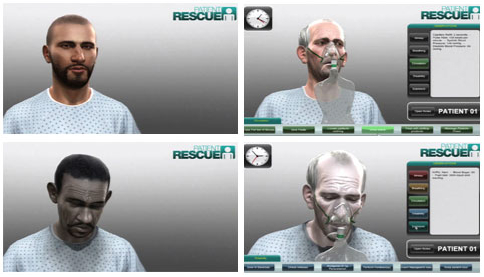
\includegraphics[scale=0.5]{tics/images/patient_side.jpg}
\caption{Evolución de un paciente en Triage}
\label{fig:triage_patient1}
\end{figure}

Al finalizar cada simulación los jugadores reciben retroalimentación acerca de
su rendimiento, incluyendo la precisión de sus chequeos, si los pacientes fueron
priorizados en el orden correcto y el tiempo que les llevó completar el triage,
en comparación con la de un experto.

La retroalimentación de los participantes que utilizaron Triage Trainer sugiere
que el mismo cumplió exitosamente sus fines. Los jugadores asociaron su
experiencia de juego con su experiencia en el mundo real y muchos de ellos
sentían que realmente estaban allí. Se espera que los jugadores puedan tomar
decisiones bajo presión, lo que ayudará a su desarrollo cognitivo. También se
observó que los jugadores tienden a discutir sus experiencias con sus compañeros
de curso, lo que también podría tener un impacto en su aprendizaje.

Un elemento que no fue evaluado por \emph{TruSim} debido a que no era
logísticamente posible fue el impacto de las pruebas en la retención del
conocimiento y el cambio de comportamiento de los
jugadores\cite{education:games}. 


\subsection{Caso 2 SimVenture}

\begin{description}
\item[Tipo:] Juego de simulación de negocios.
\item[Destinatarios:] Personas de 14 a 30 años.
\item[Contenido:] Las realidades de la creación y funcionamiento de un negocio.
\item[Desarrollador:] \emph{Venture Simulations.}
\end{description}

En el inicio del juego (ver~\ref{fig:simventure_tutorial}), a los jugadores se
les brinda informaciones y antecedentes para que que se ubiquen en escena. Ellos
deben empezar a dirigir su propio negocio en su casa de fabricación y venta de
computadoras, mientras deben mantener un trabajo de tiempo completo
independiente. El juego lleva a los jugadores a la ejecución de un negocio en su
propia casa y a la extensión del mismo a más locales, lo que requiere
contratación de personal. Los jugadores son capaces de avanzar en el juego a
través del aprendizaje de los elementos importantes de la empresa, organizadas
en cuatro categorías: organización, ventas/marketing, finanzas y operaciones.
Los jugadores toman decisiones acerca de las actividades dentro de estas áreas y
observan los resultados de sus acciones. 

\begin{figure}[h!]
\centering 
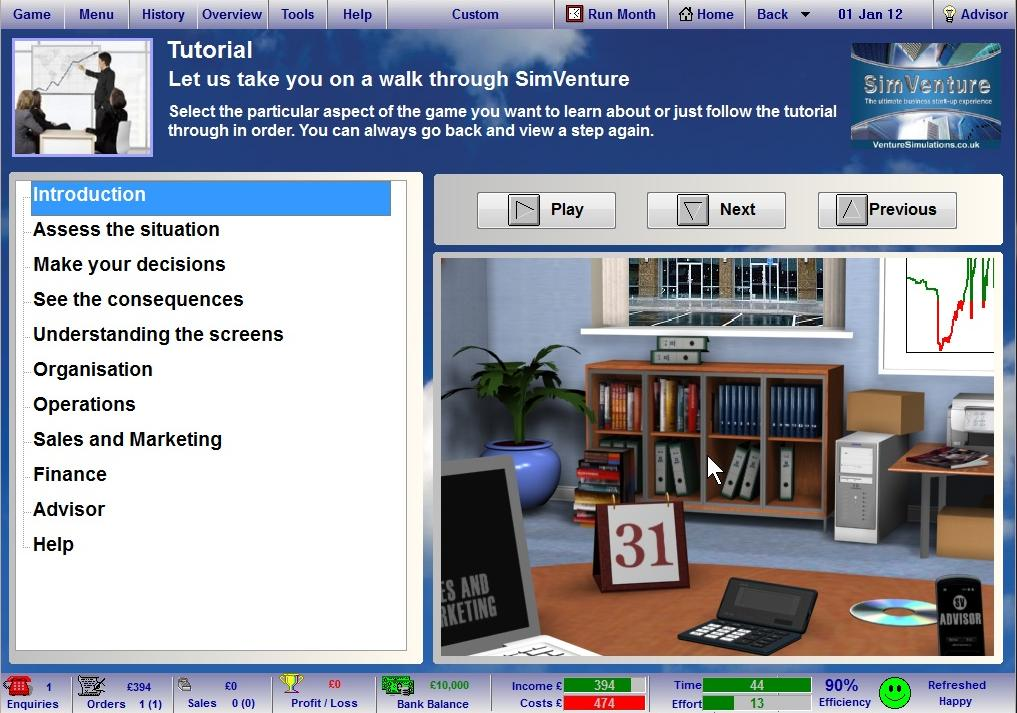
\includegraphics[scale=0.5]{tics/images/simventure-tutorial.jpg}
\caption{Tutorial de SimVenture}
\label{fig:simventure_tutorial}
\end{figure}

Los jugadores obtienen retroalimentación sobre un número de diferentes
parámetros. En un nivel básico, se puede simplemente revisar la cantidad de
ingresos que están generando. Además de esto, el éxito puede ser medido por la
cantidad de pedidos que han recibido para sus productos. También se proporciona
retroalimentación visual para representar la eficiencia de la organización y su
felicidad como individuo.

\emph{Phil Warren}, director de estudios de negocios en \emph{Snaith School}, ha
utilizado \emph{SimVenture} como complemento al plan de estudios. Según el
mismo, el plan de estudios por lo general sólo requiere que los estudiantes
aprendan sobre los diversos elementos del negocio de forma aislada, sin embargo
en la realidad, cualquier decisión que se tome en una de las partes de un
negocio tiene efecto en las demás. \emph{SimVenture} se vio como una oportunidad
de aplicar los conocimientos aprendidos en clase en una actividad práctica,
además se observó que permitir que los estudiantes jueguen en pares da un
espacio para la discusión en torno a las decisiones y aprenden de sus errores
juntos\cite{education:games}.
